\documentclass[1p]{elsarticle_modified}
%\bibliographystyle{elsarticle-num}

%\usepackage[colorlinks]{hyperref}
%\usepackage{abbrmath_seonhwa} %\Abb, \Ascr, \Acal ,\Abf, \Afrak
\usepackage{amsfonts}
\usepackage{amssymb}
\usepackage{amsmath}
\usepackage{amsthm}
\usepackage{scalefnt}
\usepackage{amsbsy}
\usepackage{kotex}
\usepackage{caption}
\usepackage{subfig}
\usepackage{color}
\usepackage{graphicx}
\usepackage{xcolor} %% white, black, red, green, blue, cyan, magenta, yellow
\usepackage{float}
\usepackage{setspace}
\usepackage{hyperref}

\usepackage{tikz}
\usetikzlibrary{arrows}

\usepackage{multirow}
\usepackage{array} % fixed length table
\usepackage{hhline}

%%%%%%%%%%%%%%%%%%%%%
\makeatletter
\renewcommand*\env@matrix[1][\arraystretch]{%
	\edef\arraystretch{#1}%
	\hskip -\arraycolsep
	\let\@ifnextchar\new@ifnextchar
	\array{*\c@MaxMatrixCols c}}
\makeatother %https://tex.stackexchange.com/questions/14071/how-can-i-increase-the-line-spacing-in-a-matrix
%%%%%%%%%%%%%%%

\usepackage[normalem]{ulem}

\newcommand{\msout}[1]{\ifmmode\text{\sout{\ensuremath{#1}}}\else\sout{#1}\fi}
%SOURCE: \msout is \stkout macro in https://tex.stackexchange.com/questions/20609/strikeout-in-math-mode

\newcommand{\cancel}[1]{
	\ifmmode
	{\color{red}\msout{#1}}
	\else
	{\color{red}\sout{#1}}
	\fi
}

\newcommand{\add}[1]{
	{\color{blue}\uwave{#1}}
}

\newcommand{\replace}[2]{
	\ifmmode
	{\color{red}\msout{#1}}{\color{blue}\uwave{#2}}
	\else
	{\color{red}\sout{#1}}{\color{blue}\uwave{#2}}
	\fi
}

\newcommand{\Sol}{\mathcal{S}} %segment
\newcommand{\D}{D} %diagram
\newcommand{\A}{\mathcal{A}} %arc


%%%%%%%%%%%%%%%%%%%%%%%%%%%%%5 test

\def\sl{\operatorname{\textup{SL}}(2,\Cbb)}
\def\psl{\operatorname{\textup{PSL}}(2,\Cbb)}
\def\quan{\mkern 1mu \triangleright \mkern 1mu}

\theoremstyle{definition}
\newtheorem{thm}{Theorem}[section]
\newtheorem{prop}[thm]{Proposition}
\newtheorem{lem}[thm]{Lemma}
\newtheorem{ques}[thm]{Question}
\newtheorem{cor}[thm]{Corollary}
\newtheorem{defn}[thm]{Definition}
\newtheorem{exam}[thm]{Example}
\newtheorem{rmk}[thm]{Remark}
\newtheorem{alg}[thm]{Algorithm}

\newcommand{\I}{\sqrt{-1}}
\begin{document}

%\begin{frontmatter}
%
%\title{Boundary parabolic representations of knots up to 8 crossings}
%
%%% Group authors per affiliation:
%\author{Yunhi Cho} 
%\address{Department of Mathematics, University of Seoul, Seoul, Korea}
%\ead{yhcho@uos.ac.kr}
%
%
%\author{Seonhwa Kim} %\fnref{s_kim}}
%\address{Center for Geometry and Physics, Institute for Basic Science, Pohang, 37673, Korea}
%\ead{ryeona17@ibs.re.kr}
%
%\author{Hyuk Kim}
%\address{Department of Mathematical Sciences, Seoul National University, Seoul 08826, Korea}
%\ead{hyukkim@snu.ac.kr}
%
%\author{Seokbeom Yoon}
%\address{Department of Mathematical Sciences, Seoul National University, Seoul, 08826,  Korea}
%\ead{sbyoon15@snu.ac.kr}
%
%\begin{abstract}
%We find all boundary parabolic representation of knots up to 8 crossings.
%
%\end{abstract}
%\begin{keyword}
%    \MSC[2010] 57M25 
%\end{keyword}
%
%\end{frontmatter}

%\linenumbers
%\tableofcontents
%
\newcommand\colored[1]{\textcolor{white}{\rule[-0.35ex]{0.8em}{1.4ex}}\kern-0.8em\color{red} #1}%
%\newcommand\colored[1]{\textcolor{white}{ #1}\kern-2.17ex	\textcolor{white}{ #1}\kern-1.81ex	\textcolor{white}{ #1}\kern-2.15ex\color{red}#1	}

{\Large $\underline{12a_{0051}~(K12a_{0051})}$}

\setlength{\tabcolsep}{10pt}
\renewcommand{\arraystretch}{1.6}
\vspace{1cm}\begin{tabular}{m{100pt}>{\centering\arraybackslash}m{274pt}}
\multirow{5}{120pt}{
	\centering
	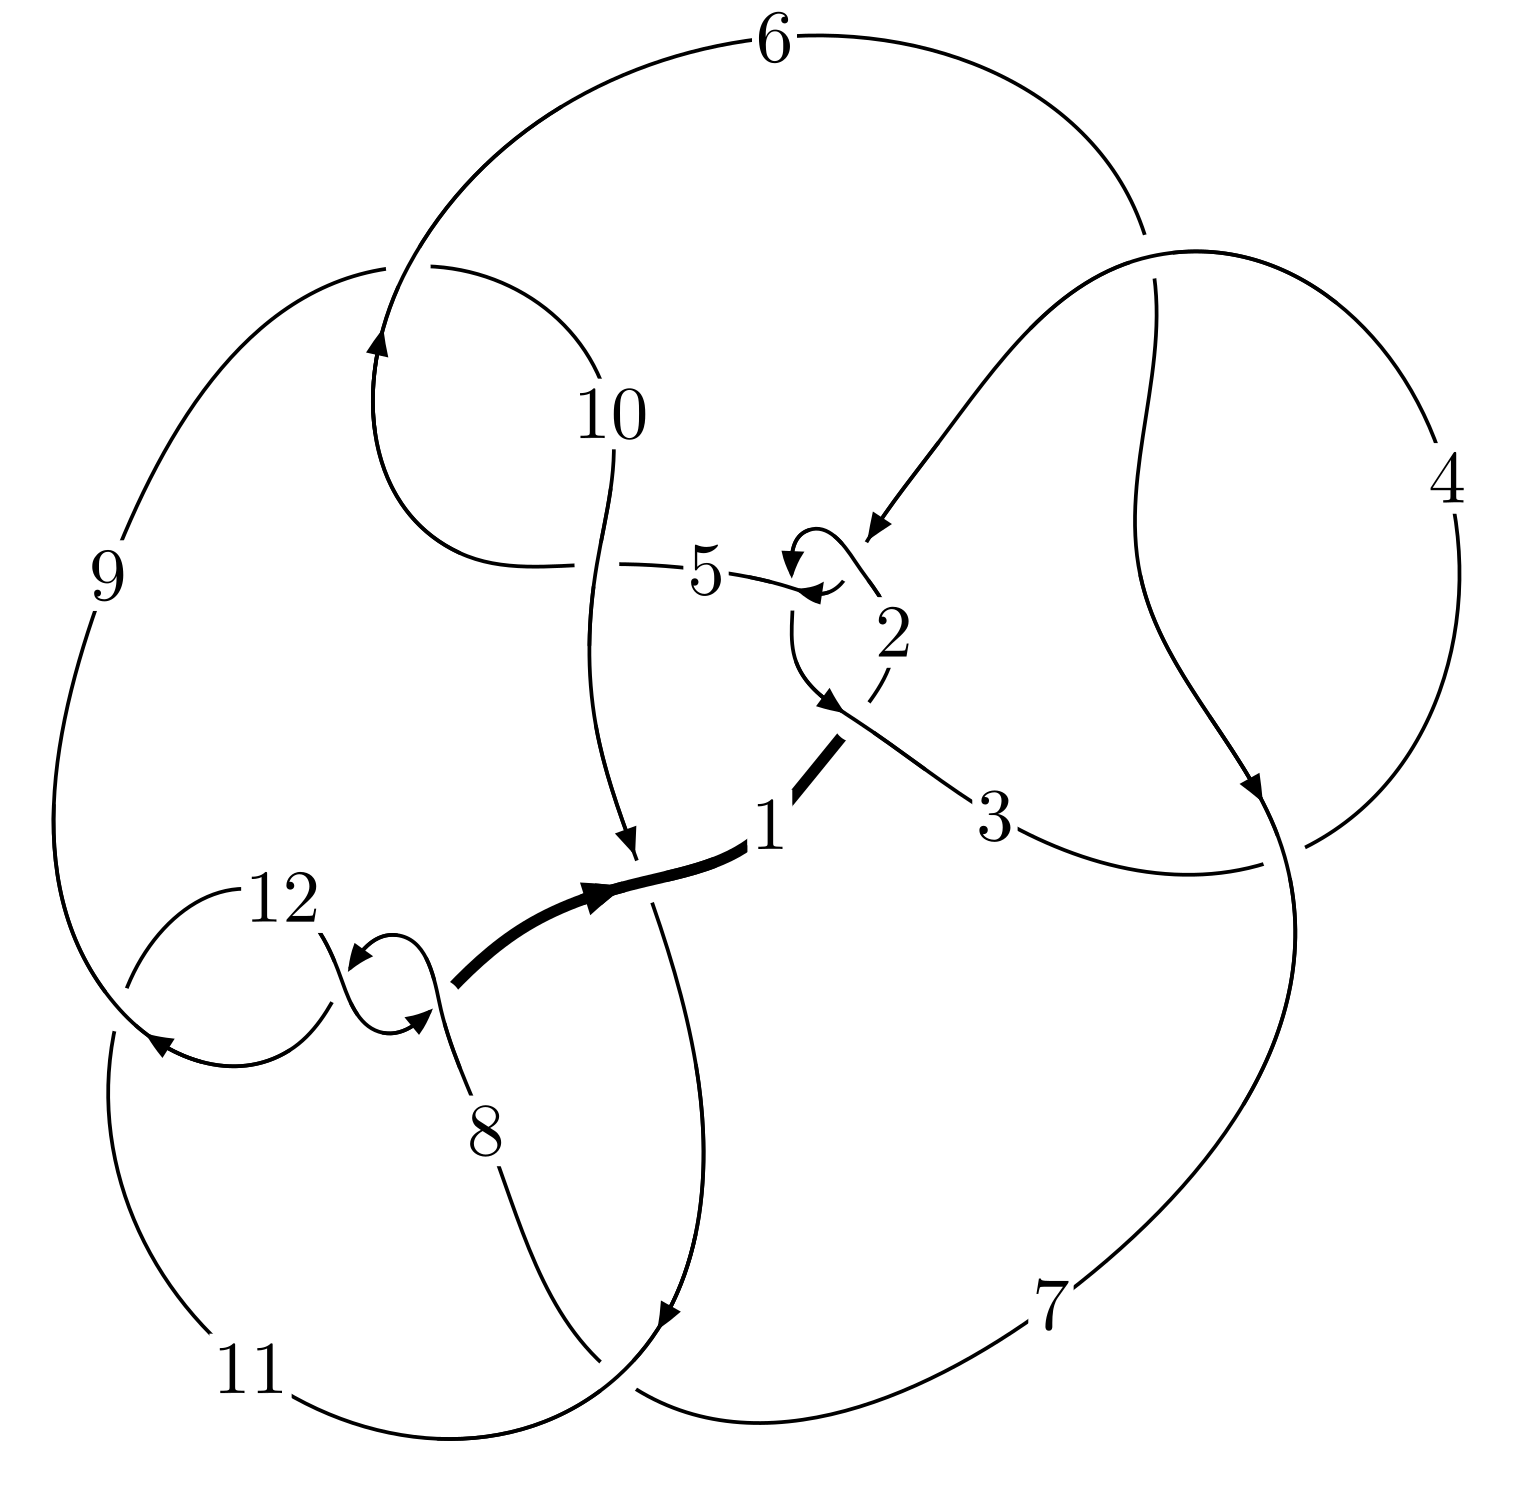
\includegraphics[width=112pt]{../../../GIT/diagram.site/Diagrams/png/852_12a_0051.png}\\
\ \ \ A knot diagram\footnotemark}&
\allowdisplaybreaks
\textbf{Linearized knot diagam} \\
\cline{2-2}
 &
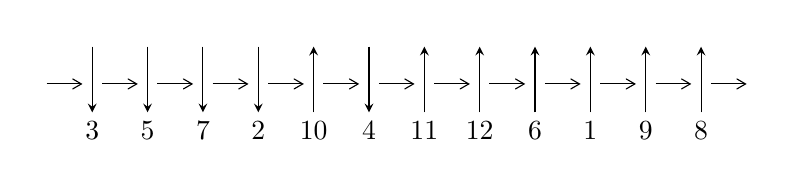
\begin{tikzpicture}[x=20pt, y=17pt]
	% nodes
	\node (C0) at (0, 0) {};
	\node (C1) at (1, 0) {};
	\node (C1U) at (1, +1) {};
	\node (C1D) at (1, -1) {3};

	\node (C2) at (2, 0) {};
	\node (C2U) at (2, +1) {};
	\node (C2D) at (2, -1) {5};

	\node (C3) at (3, 0) {};
	\node (C3U) at (3, +1) {};
	\node (C3D) at (3, -1) {7};

	\node (C4) at (4, 0) {};
	\node (C4U) at (4, +1) {};
	\node (C4D) at (4, -1) {2};

	\node (C5) at (5, 0) {};
	\node (C5U) at (5, +1) {};
	\node (C5D) at (5, -1) {10};

	\node (C6) at (6, 0) {};
	\node (C6U) at (6, +1) {};
	\node (C6D) at (6, -1) {4};

	\node (C7) at (7, 0) {};
	\node (C7U) at (7, +1) {};
	\node (C7D) at (7, -1) {11};

	\node (C8) at (8, 0) {};
	\node (C8U) at (8, +1) {};
	\node (C8D) at (8, -1) {12};

	\node (C9) at (9, 0) {};
	\node (C9U) at (9, +1) {};
	\node (C9D) at (9, -1) {6};

	\node (C10) at (10, 0) {};
	\node (C10U) at (10, +1) {};
	\node (C10D) at (10, -1) {1};

	\node (C11) at (11, 0) {};
	\node (C11U) at (11, +1) {};
	\node (C11D) at (11, -1) {9};

	\node (C12) at (12, 0) {};
	\node (C12U) at (12, +1) {};
	\node (C12D) at (12, -1) {8};
	\node (C13) at (13, 0) {};

	% arrows
	\draw[->,>={angle 60}]
	(C0) edge (C1) (C1) edge (C2) (C2) edge (C3) (C3) edge (C4) (C4) edge (C5) (C5) edge (C6) (C6) edge (C7) (C7) edge (C8) (C8) edge (C9) (C9) edge (C10) (C10) edge (C11) (C11) edge (C12) (C12) edge (C13) ;	\draw[->,>=stealth]
	(C1U) edge (C1D) (C2U) edge (C2D) (C3U) edge (C3D) (C4U) edge (C4D) (C5D) edge (C5U) (C6U) edge (C6D) (C7D) edge (C7U) (C8D) edge (C8U) (C9D) edge (C9U) (C10D) edge (C10U) (C11D) edge (C11U) (C12D) edge (C12U) ;
	\end{tikzpicture} \\
\hhline{~~} \\& 
\textbf{Solving Sequence} \\ \cline{2-2} 
 &
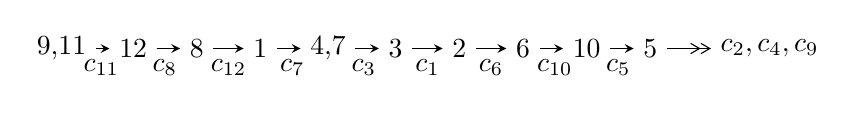
\begin{tikzpicture}[x=23pt, y=7pt]
	% node
	\node (A0) at (-1/8, 0) {9,11};
	\node (A1) at (1, 0) {12};
	\node (A2) at (2, 0) {8};
	\node (A3) at (3, 0) {1};
	\node (A4) at (65/16, 0) {4,7};
	\node (A5) at (41/8, 0) {3};
	\node (A6) at (49/8, 0) {2};
	\node (A7) at (57/8, 0) {6};
	\node (A8) at (65/8, 0) {10};
	\node (A9) at (73/8, 0) {5};
	\node (C1) at (1/2, -1) {$c_{11}$};
	\node (C2) at (3/2, -1) {$c_{8}$};
	\node (C3) at (5/2, -1) {$c_{12}$};
	\node (C4) at (7/2, -1) {$c_{7}$};
	\node (C5) at (37/8, -1) {$c_{3}$};
	\node (C6) at (45/8, -1) {$c_{1}$};
	\node (C7) at (53/8, -1) {$c_{6}$};
	\node (C8) at (61/8, -1) {$c_{10}$};
	\node (C9) at (69/8, -1) {$c_{5}$};
	\node (A10) at (11, 0) {$c_{2},c_{4},c_{9}$};

	% edge
	\draw[->,>=stealth]	
	(A0) edge (A1) (A1) edge (A2) (A2) edge (A3) (A3) edge (A4) (A4) edge (A5) (A5) edge (A6) (A6) edge (A7) (A7) edge (A8) (A8) edge (A9) ;
	\draw[->>,>={angle 60}]	
	(A9) edge (A10);
\end{tikzpicture} \\ 

\end{tabular} \\

\footnotetext{
The image of knot diagram is generated by the software ``\textbf{Draw programme}" developed by Andrew Bartholomew(\url{http://www.layer8.co.uk/maths/draw/index.htm\#Running-draw}), where we modified some parts for our purpose(\url{https://github.com/CATsTAILs/LinksPainter}).
}\phantom \\ \newline 
\centering \textbf{Ideals for irreducible components\footnotemark of $X_{\text{par}}$} 
 
\begin{align*}
I^u_{1}&=\langle 
5.08396\times10^{34} u^{109}+2.87987\times10^{35} u^{108}+\cdots+2.07043\times10^{34} b+1.00700\times10^{35},\\
\phantom{I^u_{1}}&\phantom{= \langle  }-2.40150\times10^{34} u^{109}-7.91502\times10^{34} u^{108}+\cdots+2.07043\times10^{34} a-1.21324\times10^{35},\\
\phantom{I^u_{1}}&\phantom{= \langle  }u^{110}+5 u^{109}+\cdots-7 u+1\rangle \\
I^u_{2}&=\langle 
a u- u^2+b+a,\;- u^2 a+a^2+1,\;u^3- u^2+2 u-1\rangle \\
I^u_{3}&=\langle 
- u^2+b- u-2,\;2 u^2+a+u+4,\;u^3+2 u-1\rangle \\
I^u_{4}&=\langle 
- u^2+b,\;- u^3+a- u,\;u^4+u^3+2 u^2+2 u+1\rangle \\
I^u_{5}&=\langle 
u^2+b+u,\;- u^2+a-2,\;u^3- u^2+2 u-1\rangle \\
\\
\end{align*}
\raggedright * 5 irreducible components of $\dim_{\mathbb{C}}=0$, with total 126 representations.\\
\footnotetext{All coefficients of polynomials are rational numbers. But the coefficients are sometimes approximated in decimal forms when there is not enough margin.}
\newpage
\renewcommand{\arraystretch}{1}
\centering \section*{I. $I^u_{1}= \langle 5.08\times10^{34} u^{109}+2.88\times10^{35} u^{108}+\cdots+2.07\times10^{34} b+1.01\times10^{35},\;-2.40\times10^{34} u^{109}-7.92\times10^{34} u^{108}+\cdots+2.07\times10^{34} a-1.21\times10^{35},\;u^{110}+5 u^{109}+\cdots-7 u+1 \rangle$}
\flushleft \textbf{(i) Arc colorings}\\
\begin{tabular}{m{7pt} m{180pt} m{7pt} m{180pt} }
\flushright $a_{9}=$&$\begin{pmatrix}0\\u\end{pmatrix}$ \\
\flushright $a_{11}=$&$\begin{pmatrix}1\\0\end{pmatrix}$ \\
\flushright $a_{12}=$&$\begin{pmatrix}1\\- u^2\end{pmatrix}$ \\
\flushright $a_{8}=$&$\begin{pmatrix}- u\\u^3+u\end{pmatrix}$ \\
\flushright $a_{1}=$&$\begin{pmatrix}u^2+1\\- u^4-2 u^2\end{pmatrix}$ \\
\flushright $a_{4}=$&$\begin{pmatrix}1.15991 u^{109}+3.82290 u^{108}+\cdots+17.5984 u+5.85986\\-2.45551 u^{109}-13.9096 u^{108}+\cdots+31.6055 u-4.86375\end{pmatrix}$ \\
\flushright $a_{7}=$&$\begin{pmatrix}- u^3-2 u\\u^3+u\end{pmatrix}$ \\
\flushright $a_{3}=$&$\begin{pmatrix}1.25426 u^{109}+2.47074 u^{108}+\cdots+28.5308 u+4.84333\\-4.21354 u^{109}-19.7876 u^{108}+\cdots+21.4988 u-3.81138\end{pmatrix}$ \\
\flushright $a_{2}=$&$\begin{pmatrix}-1.32122 u^{109}-5.24754 u^{108}+\cdots-10.3151 u-3.64345\\0.442881 u^{109}+4.21484 u^{108}+\cdots-18.3658 u+2.99673\end{pmatrix}$ \\
\flushright $a_{6}=$&$\begin{pmatrix}-3.93346 u^{109}-15.5438 u^{108}+\cdots+29.5005 u-0.0441834\\4.97771 u^{109}+20.9442 u^{108}+\cdots-6.60421 u+0.827017\end{pmatrix}$ \\
\flushright $a_{10}=$&$\begin{pmatrix}- u^6-3 u^4-2 u^2+1\\u^8+4 u^6+4 u^4\end{pmatrix}$ \\
\flushright $a_{5}=$&$\begin{pmatrix}-1.46652 u^{109}-8.11160 u^{108}+\cdots+30.3922 u+0.400062\\0.0103310 u^{109}+0.286370 u^{108}+\cdots-2.69149 u+0.0323288\end{pmatrix}$\\&\end{tabular}
\flushleft \textbf{(ii) Obstruction class $= -1$}\\~\\
\flushleft \textbf{(iii) Cusp Shapes $= 1.61410 u^{109}+7.48255 u^{108}+\cdots-53.0640 u-4.23776$}\\~\\
\newpage\renewcommand{\arraystretch}{1}
\flushleft \textbf{(iv) u-Polynomials at the component}\newline \\
\begin{tabular}{m{50pt}|m{274pt}}
Crossings & \hspace{64pt}u-Polynomials at each crossing \\
\hline $$\begin{aligned}c_{1}\end{aligned}$$&$\begin{aligned}
&u^{110}+53 u^{109}+\cdots+874 u+1
\end{aligned}$\\
\hline $$\begin{aligned}c_{2},c_{4}\end{aligned}$$&$\begin{aligned}
&u^{110}-11 u^{109}+\cdots+20 u+1
\end{aligned}$\\
\hline $$\begin{aligned}c_{3},c_{6}\end{aligned}$$&$\begin{aligned}
&u^{110}-4 u^{109}+\cdots+1344 u-128
\end{aligned}$\\
\hline $$\begin{aligned}c_{5},c_{9}\end{aligned}$$&$\begin{aligned}
&u^{110}-2 u^{109}+\cdots-1024 u-512
\end{aligned}$\\
\hline $$\begin{aligned}c_{7}\end{aligned}$$&$\begin{aligned}
&u^{110}-5 u^{109}+\cdots-3176 u+292
\end{aligned}$\\
\hline $$\begin{aligned}c_{8},c_{11},c_{12}\end{aligned}$$&$\begin{aligned}
&u^{110}+5 u^{109}+\cdots-7 u+1
\end{aligned}$\\
\hline $$\begin{aligned}c_{10}\end{aligned}$$&$\begin{aligned}
&u^{110}+23 u^{109}+\cdots-3335609 u+61891
\end{aligned}$\\
\hline
\end{tabular}\\~\\
\newpage\renewcommand{\arraystretch}{1}
\flushleft \textbf{(v) Riley Polynomials at the component}\newline \\
\begin{tabular}{m{50pt}|m{274pt}}
Crossings & \hspace{64pt}Riley Polynomials at each crossing \\
\hline $$\begin{aligned}c_{1}\end{aligned}$$&$\begin{aligned}
&y^{110}+19 y^{109}+\cdots-806974 y+1
\end{aligned}$\\
\hline $$\begin{aligned}c_{2},c_{4}\end{aligned}$$&$\begin{aligned}
&y^{110}-53 y^{109}+\cdots-874 y+1
\end{aligned}$\\
\hline $$\begin{aligned}c_{3},c_{6}\end{aligned}$$&$\begin{aligned}
&y^{110}+54 y^{109}+\cdots-192512 y+16384
\end{aligned}$\\
\hline $$\begin{aligned}c_{5},c_{9}\end{aligned}$$&$\begin{aligned}
&y^{110}+56 y^{109}+\cdots+2228224 y+262144
\end{aligned}$\\
\hline $$\begin{aligned}c_{7}\end{aligned}$$&$\begin{aligned}
&y^{110}+9 y^{109}+\cdots-11413240 y+85264
\end{aligned}$\\
\hline $$\begin{aligned}c_{8},c_{11},c_{12}\end{aligned}$$&$\begin{aligned}
&y^{110}+101 y^{109}+\cdots-147 y+1
\end{aligned}$\\
\hline $$\begin{aligned}c_{10}\end{aligned}$$&$\begin{aligned}
&y^{110}+41 y^{109}+\cdots-17639818908843 y+3830495881
\end{aligned}$\\
\hline
\end{tabular}\\~\\
\newpage\flushleft \textbf{(vi) Complex Volumes and Cusp Shapes}
$$\begin{array}{c|c|c}  
\text{Solutions to }I^u_{1}& \I (\text{vol} + \sqrt{-1}CS) & \text{Cusp shape}\\
 \hline 
\begin{aligned}
u &= -0.087769 + 1.071150 I \\
a &= -1.248980 - 0.465454 I \\
b &= -1.37873 - 0.37865 I\end{aligned}
 & \phantom{-}2.25688 + 0.90789 I & \phantom{-0.000000 } 0 \\ \hline\begin{aligned}
u &= -0.087769 - 1.071150 I \\
a &= -1.248980 + 0.465454 I \\
b &= -1.37873 + 0.37865 I\end{aligned}
 & \phantom{-}2.25688 - 0.90789 I & \phantom{-0.000000 } 0 \\ \hline\begin{aligned}
u &= \phantom{-}0.267272 + 1.065890 I \\
a &= -1.50466 - 0.67505 I \\
b &= -0.984660 + 0.847043 I\end{aligned}
 & \phantom{-}1.22660 + 4.08841 I & \phantom{-0.000000 } 0 \\ \hline\begin{aligned}
u &= \phantom{-}0.267272 - 1.065890 I \\
a &= -1.50466 + 0.67505 I \\
b &= -0.984660 - 0.847043 I\end{aligned}
 & \phantom{-}1.22660 - 4.08841 I & \phantom{-0.000000 } 0 \\ \hline\begin{aligned}
u &= -0.467803 + 0.703618 I \\
a &= \phantom{-}2.29074 - 0.39775 I \\
b &= -0.223957 + 0.915152 I\end{aligned}
 & -2.03455 + 9.47276 I & \phantom{-0.000000 } 0 \\ \hline\begin{aligned}
u &= -0.467803 - 0.703618 I \\
a &= \phantom{-}2.29074 + 0.39775 I \\
b &= -0.223957 - 0.915152 I\end{aligned}
 & -2.03455 - 9.47276 I & \phantom{-0.000000 } 0 \\ \hline\begin{aligned}
u &= \phantom{-}0.326859 + 1.111260 I \\
a &= \phantom{-}1.47565 + 0.59737 I \\
b &= \phantom{-}0.842871 - 0.962044 I\end{aligned}
 & -0.76167 + 9.32773 I & \phantom{-0.000000 } 0 \\ \hline\begin{aligned}
u &= \phantom{-}0.326859 - 1.111260 I \\
a &= \phantom{-}1.47565 - 0.59737 I \\
b &= \phantom{-}0.842871 + 0.962044 I\end{aligned}
 & -0.76167 - 9.32773 I & \phantom{-0.000000 } 0 \\ \hline\begin{aligned}
u &= \phantom{-}0.044918 + 1.159940 I \\
a &= \phantom{-}0.485785 + 0.353856 I \\
b &= \phantom{-}0.012116 - 1.098570 I\end{aligned}
 & -2.74728 + 0.22494 I & \phantom{-0.000000 } 0 \\ \hline\begin{aligned}
u &= \phantom{-}0.044918 - 1.159940 I \\
a &= \phantom{-}0.485785 - 0.353856 I \\
b &= \phantom{-}0.012116 + 1.098570 I\end{aligned}
 & -2.74728 - 0.22494 I & \phantom{-0.000000 } 0\\
 \hline 
 \end{array}$$\newpage$$\begin{array}{c|c|c}  
\text{Solutions to }I^u_{1}& \I (\text{vol} + \sqrt{-1}CS) & \text{Cusp shape}\\
 \hline 
\begin{aligned}
u &= \phantom{-}0.213857 + 1.147760 I \\
a &= -0.609333 - 0.547444 I \\
b &= -0.276527 + 1.333880 I\end{aligned}
 & -3.24169 + 3.96546 I & \phantom{-0.000000 } 0 \\ \hline\begin{aligned}
u &= \phantom{-}0.213857 - 1.147760 I \\
a &= -0.609333 + 0.547444 I \\
b &= -0.276527 - 1.333880 I\end{aligned}
 & -3.24169 - 3.96546 I & \phantom{-0.000000 } 0 \\ \hline\begin{aligned}
u &= -0.122184 + 1.171470 I \\
a &= \phantom{-}0.937221 + 0.413575 I \\
b &= \phantom{-}1.70265 + 0.66436 I\end{aligned}
 & \phantom{-}1.13228 - 4.77677 I & \phantom{-0.000000 } 0 \\ \hline\begin{aligned}
u &= -0.122184 - 1.171470 I \\
a &= \phantom{-}0.937221 - 0.413575 I \\
b &= \phantom{-}1.70265 - 0.66436 I\end{aligned}
 & \phantom{-}1.13228 + 4.77677 I & \phantom{-0.000000 } 0 \\ \hline\begin{aligned}
u &= -0.751985 + 0.316865 I \\
a &= -0.19275 - 2.67863 I \\
b &= \phantom{-}0.28939 + 2.30634 I\end{aligned}
 & -0.69158 - 13.75370 I & \phantom{-0.000000 -}0. + 9.91597 I \\ \hline\begin{aligned}
u &= -0.751985 - 0.316865 I \\
a &= -0.19275 + 2.67863 I \\
b &= \phantom{-}0.28939 - 2.30634 I\end{aligned}
 & -0.69158 + 13.75370 I & \phantom{-0.000000 } 0. - 9.91597 I \\ \hline\begin{aligned}
u &= -0.682778 + 0.437855 I \\
a &= \phantom{-}0.140125 + 0.021845 I \\
b &= \phantom{-}0.306524 - 0.099329 I\end{aligned}
 & -4.92429 - 1.07894 I & \phantom{-0.000000 } 0 \\ \hline\begin{aligned}
u &= -0.682778 - 0.437855 I \\
a &= \phantom{-}0.140125 - 0.021845 I \\
b &= \phantom{-}0.306524 + 0.099329 I\end{aligned}
 & -4.92429 + 1.07894 I & \phantom{-0.000000 } 0 \\ \hline\begin{aligned}
u &= -0.608747 + 0.529637 I \\
a &= -0.156738 + 0.093345 I \\
b &= -0.147370 + 0.361143 I\end{aligned}
 & -5.26321 - 3.26086 I & \phantom{-0.000000 -}0. + 8.42000 I \\ \hline\begin{aligned}
u &= -0.608747 - 0.529637 I \\
a &= -0.156738 - 0.093345 I \\
b &= -0.147370 - 0.361143 I\end{aligned}
 & -5.26321 + 3.26086 I & \phantom{-0.000000 } 0. - 8.42000 I\\
 \hline 
 \end{array}$$\newpage$$\begin{array}{c|c|c}  
\text{Solutions to }I^u_{1}& \I (\text{vol} + \sqrt{-1}CS) & \text{Cusp shape}\\
 \hline 
\begin{aligned}
u &= \phantom{-}0.133764 + 1.201670 I \\
a &= \phantom{-}1.70456 + 1.05818 I \\
b &= \phantom{-}2.18770 - 1.16206 I\end{aligned}
 & -4.25280 + 2.01271 I & \phantom{-0.000000 } 0 \\ \hline\begin{aligned}
u &= \phantom{-}0.133764 - 1.201670 I \\
a &= \phantom{-}1.70456 - 1.05818 I \\
b &= \phantom{-}2.18770 + 1.16206 I\end{aligned}
 & -4.25280 - 2.01271 I & \phantom{-0.000000 } 0 \\ \hline\begin{aligned}
u &= -0.393997 + 0.682907 I \\
a &= -2.30080 + 0.11323 I \\
b &= \phantom{-}0.155381 - 0.647926 I\end{aligned}
 & \phantom{-}0.47353 + 4.02638 I & \phantom{-}2.00000 - 1.65162 I \\ \hline\begin{aligned}
u &= -0.393997 - 0.682907 I \\
a &= -2.30080 - 0.11323 I \\
b &= \phantom{-}0.155381 + 0.647926 I\end{aligned}
 & \phantom{-}0.47353 - 4.02638 I & \phantom{-}2.00000 + 1.65162 I \\ \hline\begin{aligned}
u &= -0.728838 + 0.296790 I \\
a &= \phantom{-}0.43006 + 2.61474 I \\
b &= -0.35716 - 2.24164 I\end{aligned}
 & \phantom{-}1.88370 - 8.04851 I & \phantom{-}4.66389 + 6.64940 I \\ \hline\begin{aligned}
u &= -0.728838 - 0.296790 I \\
a &= \phantom{-}0.43006 - 2.61474 I \\
b &= -0.35716 + 2.24164 I\end{aligned}
 & \phantom{-}1.88370 + 8.04851 I & \phantom{-}4.66389 - 6.64940 I \\ \hline\begin{aligned}
u &= \phantom{-}0.777005 + 0.085415 I \\
a &= -0.01227 + 2.08995 I \\
b &= -0.29493 - 1.78626 I\end{aligned}
 & \phantom{-}2.37677 - 5.29652 I & \phantom{-}3.30695 + 5.27195 I \\ \hline\begin{aligned}
u &= \phantom{-}0.777005 - 0.085415 I \\
a &= -0.01227 - 2.08995 I \\
b &= -0.29493 + 1.78626 I\end{aligned}
 & \phantom{-}2.37677 + 5.29652 I & \phantom{-}3.30695 - 5.27195 I \\ \hline\begin{aligned}
u &= -0.702649 + 0.316627 I \\
a &= \phantom{-}0.203452 + 0.089662 I \\
b &= \phantom{-}0.504761 + 0.070122 I\end{aligned}
 & -2.93391 - 7.17237 I & \phantom{-0.000000 -}0. + 7.42213 I \\ \hline\begin{aligned}
u &= -0.702649 - 0.316627 I \\
a &= \phantom{-}0.203452 - 0.089662 I \\
b &= \phantom{-}0.504761 - 0.070122 I\end{aligned}
 & -2.93391 + 7.17237 I & \phantom{-0.000000 } 0. - 7.42213 I\\
 \hline 
 \end{array}$$\newpage$$\begin{array}{c|c|c}  
\text{Solutions to }I^u_{1}& \I (\text{vol} + \sqrt{-1}CS) & \text{Cusp shape}\\
 \hline 
\begin{aligned}
u &= -0.676292 + 0.325580 I \\
a &= -0.92125 - 3.03516 I \\
b &= \phantom{-}0.62862 + 2.30011 I\end{aligned}
 & -3.81916 - 4.42307 I & \phantom{-}0.33207 + 6.45804 I \\ \hline\begin{aligned}
u &= -0.676292 - 0.325580 I \\
a &= -0.92125 + 3.03516 I \\
b &= \phantom{-}0.62862 - 2.30011 I\end{aligned}
 & -3.81916 + 4.42307 I & \phantom{-}0.33207 - 6.45804 I \\ \hline\begin{aligned}
u &= \phantom{-}0.737560 + 0.128821 I \\
a &= -0.23433 - 2.21989 I \\
b &= \phantom{-}0.34707 + 1.87285 I\end{aligned}
 & \phantom{-}4.05943 - 0.32957 I & \phantom{-}7.05242 + 0.19707 I \\ \hline\begin{aligned}
u &= \phantom{-}0.737560 - 0.128821 I \\
a &= -0.23433 + 2.21989 I \\
b &= \phantom{-}0.34707 - 1.87285 I\end{aligned}
 & \phantom{-}4.05943 + 0.32957 I & \phantom{-}7.05242 - 0.19707 I \\ \hline\begin{aligned}
u &= \phantom{-}0.666718 + 0.321526 I \\
a &= \phantom{-}1.00379 + 1.71314 I \\
b &= -0.57519 - 1.79009 I\end{aligned}
 & \phantom{-}1.83773 + 7.20528 I & \phantom{-}3.32675 - 7.67477 I \\ \hline\begin{aligned}
u &= \phantom{-}0.666718 - 0.321526 I \\
a &= \phantom{-}1.00379 - 1.71314 I \\
b &= -0.57519 + 1.79009 I\end{aligned}
 & \phantom{-}1.83773 - 7.20528 I & \phantom{-}3.32675 + 7.67477 I \\ \hline\begin{aligned}
u &= -0.422080 + 0.598409 I \\
a &= -0.305176 + 0.223190 I \\
b &= -0.003864 + 0.654541 I\end{aligned}
 & -4.06310 + 3.25446 I & -2.82924 - 1.68811 I \\ \hline\begin{aligned}
u &= -0.422080 - 0.598409 I \\
a &= -0.305176 - 0.223190 I \\
b &= -0.003864 - 0.654541 I\end{aligned}
 & -4.06310 - 3.25446 I & -2.82924 + 1.68811 I \\ \hline\begin{aligned}
u &= \phantom{-}0.673412 + 0.257531 I \\
a &= -0.90832 - 1.97279 I \\
b &= \phantom{-}0.55569 + 1.85787 I\end{aligned}
 & \phantom{-}3.75181 + 2.12756 I & \phantom{-}7.14555 - 2.70279 I \\ \hline\begin{aligned}
u &= \phantom{-}0.673412 - 0.257531 I \\
a &= -0.90832 + 1.97279 I \\
b &= \phantom{-}0.55569 - 1.85787 I\end{aligned}
 & \phantom{-}3.75181 - 2.12756 I & \phantom{-}7.14555 + 2.70279 I\\
 \hline 
 \end{array}$$\newpage$$\begin{array}{c|c|c}  
\text{Solutions to }I^u_{1}& \I (\text{vol} + \sqrt{-1}CS) & \text{Cusp shape}\\
 \hline 
\begin{aligned}
u &= -0.633760 + 0.307440 I \\
a &= -0.191099 - 0.147798 I \\
b &= -0.453297 - 0.191626 I\end{aligned}
 & -1.35364 - 2.39156 I & \phantom{-}1.35494 + 3.44541 I \\ \hline\begin{aligned}
u &= -0.633760 - 0.307440 I \\
a &= -0.191099 + 0.147798 I \\
b &= -0.453297 + 0.191626 I\end{aligned}
 & -1.35364 + 2.39156 I & \phantom{-}1.35494 - 3.44541 I \\ \hline\begin{aligned}
u &= -0.442645 + 0.534598 I \\
a &= \phantom{-}2.95117 + 0.09459 I \\
b &= -0.765044 + 0.351218 I\end{aligned}
 & -4.73490 + 0.63177 I & -2.64133 - 0.41353 I \\ \hline\begin{aligned}
u &= -0.442645 - 0.534598 I \\
a &= \phantom{-}2.95117 - 0.09459 I \\
b &= -0.765044 - 0.351218 I\end{aligned}
 & -4.73490 - 0.63177 I & -2.64133 + 0.41353 I \\ \hline\begin{aligned}
u &= \phantom{-}0.238477 + 1.301950 I \\
a &= \phantom{-}1.94233 - 0.22816 I \\
b &= -0.30674 - 2.02821 I\end{aligned}
 & -4.24078 + 2.59768 I & \phantom{-0.000000 } 0 \\ \hline\begin{aligned}
u &= \phantom{-}0.238477 - 1.301950 I \\
a &= \phantom{-}1.94233 + 0.22816 I \\
b &= -0.30674 + 2.02821 I\end{aligned}
 & -4.24078 - 2.59768 I & \phantom{-0.000000 } 0 \\ \hline\begin{aligned}
u &= \phantom{-}0.668764 + 0.067218 I \\
a &= -1.01044 - 2.15829 I \\
b &= \phantom{-}0.17342 + 1.51996 I\end{aligned}
 & -0.004153 - 0.660121 I & -0.81116 + 3.72545 I \\ \hline\begin{aligned}
u &= \phantom{-}0.668764 - 0.067218 I \\
a &= -1.01044 + 2.15829 I \\
b &= \phantom{-}0.17342 - 1.51996 I\end{aligned}
 & -0.004153 + 0.660121 I & -0.81116 - 3.72545 I \\ \hline\begin{aligned}
u &= \phantom{-}0.327530 + 1.290810 I \\
a &= -0.880564 - 0.599152 I \\
b &= -0.39051 + 2.00378 I\end{aligned}
 & -1.90814 - 1.31421 I & \phantom{-0.000000 } 0 \\ \hline\begin{aligned}
u &= \phantom{-}0.327530 - 1.290810 I \\
a &= -0.880564 + 0.599152 I \\
b &= -0.39051 - 2.00378 I\end{aligned}
 & -1.90814 + 1.31421 I & \phantom{-0.000000 } 0\\
 \hline 
 \end{array}$$\newpage$$\begin{array}{c|c|c}  
\text{Solutions to }I^u_{1}& \I (\text{vol} + \sqrt{-1}CS) & \text{Cusp shape}\\
 \hline 
\begin{aligned}
u &= \phantom{-}0.431721 + 0.498945 I \\
a &= \phantom{-}1.38512 + 1.26258 I \\
b &= \phantom{-}0.329753 - 0.717428 I\end{aligned}
 & \phantom{-}0.96271 - 3.52397 I & \phantom{-}1.82648 + 1.71517 I \\ \hline\begin{aligned}
u &= \phantom{-}0.431721 - 0.498945 I \\
a &= \phantom{-}1.38512 - 1.26258 I \\
b &= \phantom{-}0.329753 + 0.717428 I\end{aligned}
 & \phantom{-}0.96271 + 3.52397 I & \phantom{-}1.82648 - 1.71517 I \\ \hline\begin{aligned}
u &= -0.625020 + 0.195335 I \\
a &= \phantom{-}1.02317 + 1.71908 I \\
b &= -0.30780 - 1.78368 I\end{aligned}
 & \phantom{-}4.65417 - 3.79918 I & \phantom{-}5.60561 + 9.12001 I \\ \hline\begin{aligned}
u &= -0.625020 - 0.195335 I \\
a &= \phantom{-}1.02317 - 1.71908 I \\
b &= -0.30780 + 1.78368 I\end{aligned}
 & \phantom{-}4.65417 + 3.79918 I & \phantom{-}5.60561 - 9.12001 I \\ \hline\begin{aligned}
u &= \phantom{-}0.158715 + 1.337860 I \\
a &= \phantom{-}0.527912 - 0.390102 I \\
b &= -0.670480 - 0.244495 I\end{aligned}
 & -3.43387 + 2.25266 I & \phantom{-0.000000 } 0 \\ \hline\begin{aligned}
u &= \phantom{-}0.158715 - 1.337860 I \\
a &= \phantom{-}0.527912 + 0.390102 I \\
b &= -0.670480 + 0.244495 I\end{aligned}
 & -3.43387 - 2.25266 I & \phantom{-0.000000 } 0 \\ \hline\begin{aligned}
u &= \phantom{-}0.300858 + 1.330050 I \\
a &= \phantom{-}1.015650 + 0.572458 I \\
b &= \phantom{-}0.43639 - 2.22756 I\end{aligned}
 & -0.51775 + 3.42145 I & \phantom{-0.000000 } 0 \\ \hline\begin{aligned}
u &= \phantom{-}0.300858 - 1.330050 I \\
a &= \phantom{-}1.015650 - 0.572458 I \\
b &= \phantom{-}0.43639 + 2.22756 I\end{aligned}
 & -0.51775 - 3.42145 I & \phantom{-0.000000 } 0 \\ \hline\begin{aligned}
u &= \phantom{-}0.590275 + 0.237552 I \\
a &= \phantom{-}1.14216 + 1.56879 I \\
b &= \phantom{-}0.028965 - 0.993228 I\end{aligned}
 & -0.45742 + 2.08316 I & \phantom{-}1.71834 - 4.71563 I \\ \hline\begin{aligned}
u &= \phantom{-}0.590275 - 0.237552 I \\
a &= \phantom{-}1.14216 - 1.56879 I \\
b &= \phantom{-}0.028965 + 0.993228 I\end{aligned}
 & -0.45742 - 2.08316 I & \phantom{-}1.71834 + 4.71563 I\\
 \hline 
 \end{array}$$\newpage$$\begin{array}{c|c|c}  
\text{Solutions to }I^u_{1}& \I (\text{vol} + \sqrt{-1}CS) & \text{Cusp shape}\\
 \hline 
\begin{aligned}
u &= -0.448708 + 0.424163 I \\
a &= \phantom{-}0.087098 - 0.355565 I \\
b &= -0.189088 - 0.505206 I\end{aligned}
 & -2.04918 - 1.01718 I & -0.77645 + 4.39237 I \\ \hline\begin{aligned}
u &= -0.448708 - 0.424163 I \\
a &= \phantom{-}0.087098 + 0.355565 I \\
b &= -0.189088 + 0.505206 I\end{aligned}
 & -2.04918 + 1.01718 I & -0.77645 - 4.39237 I \\ \hline\begin{aligned}
u &= -0.213217 + 1.374140 I \\
a &= -0.077328 + 0.925196 I \\
b &= -1.84754 - 2.39610 I\end{aligned}
 & -0.811385 - 0.560255 I & \phantom{-0.000000 } 0 \\ \hline\begin{aligned}
u &= -0.213217 - 1.374140 I \\
a &= -0.077328 - 0.925196 I \\
b &= -1.84754 + 2.39610 I\end{aligned}
 & -0.811385 + 0.560255 I & \phantom{-0.000000 } 0 \\ \hline\begin{aligned}
u &= \phantom{-}0.232900 + 0.562056 I \\
a &= -1.68860 - 1.12075 I \\
b &= -0.368435 + 0.504187 I\end{aligned}
 & \phantom{-}2.28204 + 1.25980 I & \phantom{-}3.87420 - 3.95142 I \\ \hline\begin{aligned}
u &= \phantom{-}0.232900 - 0.562056 I \\
a &= -1.68860 + 1.12075 I \\
b &= -0.368435 - 0.504187 I\end{aligned}
 & \phantom{-}2.28204 - 1.25980 I & \phantom{-}3.87420 + 3.95142 I \\ \hline\begin{aligned}
u &= \phantom{-}0.096418 + 1.393080 I \\
a &= \phantom{-}0.667863 + 0.044755 I \\
b &= -0.504387 - 0.413403 I\end{aligned}
 & -3.56329 + 2.49031 I & \phantom{-0.000000 } 0 \\ \hline\begin{aligned}
u &= \phantom{-}0.096418 - 1.393080 I \\
a &= \phantom{-}0.667863 - 0.044755 I \\
b &= -0.504387 + 0.413403 I\end{aligned}
 & -3.56329 - 2.49031 I & \phantom{-0.000000 } 0 \\ \hline\begin{aligned}
u &= \phantom{-}0.205762 + 1.386790 I \\
a &= -1.46276 - 0.03865 I \\
b &= \phantom{-}0.01850 + 3.00217 I\end{aligned}
 & -6.10565 + 2.87492 I & \phantom{-0.000000 } 0 \\ \hline\begin{aligned}
u &= \phantom{-}0.205762 - 1.386790 I \\
a &= -1.46276 + 0.03865 I \\
b &= \phantom{-}0.01850 - 3.00217 I\end{aligned}
 & -6.10565 - 2.87492 I & \phantom{-0.000000 } 0\\
 \hline 
 \end{array}$$\newpage$$\begin{array}{c|c|c}  
\text{Solutions to }I^u_{1}& \I (\text{vol} + \sqrt{-1}CS) & \text{Cusp shape}\\
 \hline 
\begin{aligned}
u &= -0.239877 + 1.381360 I \\
a &= \phantom{-}0.363803 - 1.007460 I \\
b &= \phantom{-}1.83084 + 2.64228 I\end{aligned}
 & -0.37974 - 6.94098 I & \phantom{-0.000000 } 0 \\ \hline\begin{aligned}
u &= -0.239877 - 1.381360 I \\
a &= \phantom{-}0.363803 + 1.007460 I \\
b &= \phantom{-}1.83084 - 2.64228 I\end{aligned}
 & -0.37974 + 6.94098 I & \phantom{-0.000000 } 0 \\ \hline\begin{aligned}
u &= \phantom{-}0.23220 + 1.39528 I \\
a &= -1.080520 + 0.161583 I \\
b &= \phantom{-}0.376710 + 0.711456 I\end{aligned}
 & -5.68295 + 5.10949 I & \phantom{-0.000000 } 0 \\ \hline\begin{aligned}
u &= \phantom{-}0.23220 - 1.39528 I \\
a &= -1.080520 - 0.161583 I \\
b &= \phantom{-}0.376710 - 0.711456 I\end{aligned}
 & -5.68295 - 5.10949 I & \phantom{-0.000000 } 0 \\ \hline\begin{aligned}
u &= -0.557111 + 0.152288 I \\
a &= -1.16889 - 1.17714 I \\
b &= \phantom{-}0.13263 + 1.54331 I\end{aligned}
 & \phantom{-}4.09579 + 2.24249 I & \phantom{-}2.09249 + 6.49191 I \\ \hline\begin{aligned}
u &= -0.557111 - 0.152288 I \\
a &= -1.16889 + 1.17714 I \\
b &= \phantom{-}0.13263 - 1.54331 I\end{aligned}
 & \phantom{-}4.09579 - 2.24249 I & \phantom{-}2.09249 - 6.49191 I \\ \hline\begin{aligned}
u &= \phantom{-}0.26322 + 1.40067 I \\
a &= \phantom{-}1.150470 + 0.262478 I \\
b &= \phantom{-}0.12209 - 2.54689 I\end{aligned}
 & -1.53483 + 5.53884 I & \phantom{-0.000000 } 0 \\ \hline\begin{aligned}
u &= \phantom{-}0.26322 - 1.40067 I \\
a &= \phantom{-}1.150470 - 0.262478 I \\
b &= \phantom{-}0.12209 + 2.54689 I\end{aligned}
 & -1.53483 - 5.53884 I & \phantom{-0.000000 } 0 \\ \hline\begin{aligned}
u &= -0.24822 + 1.42034 I \\
a &= \phantom{-}0.125478 + 0.107540 I \\
b &= \phantom{-}0.746609 - 0.398952 I\end{aligned}
 & -6.88313 - 5.63183 I & \phantom{-0.000000 } 0 \\ \hline\begin{aligned}
u &= -0.24822 - 1.42034 I \\
a &= \phantom{-}0.125478 - 0.107540 I \\
b &= \phantom{-}0.746609 + 0.398952 I\end{aligned}
 & -6.88313 + 5.63183 I & \phantom{-0.000000 } 0\\
 \hline 
 \end{array}$$\newpage$$\begin{array}{c|c|c}  
\text{Solutions to }I^u_{1}& \I (\text{vol} + \sqrt{-1}CS) & \text{Cusp shape}\\
 \hline 
\begin{aligned}
u &= -0.17484 + 1.43130 I \\
a &= \phantom{-}0.024046 + 0.220816 I \\
b &= \phantom{-}0.936174 + 0.364235 I\end{aligned}
 & -7.94217 - 3.35665 I & \phantom{-0.000000 } 0 \\ \hline\begin{aligned}
u &= -0.17484 - 1.43130 I \\
a &= \phantom{-}0.024046 - 0.220816 I \\
b &= \phantom{-}0.936174 - 0.364235 I\end{aligned}
 & -7.94217 + 3.35665 I & \phantom{-0.000000 } 0 \\ \hline\begin{aligned}
u &= -0.10527 + 1.44541 I \\
a &= \phantom{-}0.853980 + 0.625681 I \\
b &= -1.59490 - 0.51909 I\end{aligned}
 & -6.16042 + 2.51482 I & \phantom{-0.000000 } 0 \\ \hline\begin{aligned}
u &= -0.10527 - 1.44541 I \\
a &= \phantom{-}0.853980 - 0.625681 I \\
b &= -1.59490 + 0.51909 I\end{aligned}
 & -6.16042 - 2.51482 I & \phantom{-0.000000 } 0 \\ \hline\begin{aligned}
u &= \phantom{-}0.16355 + 1.44140 I \\
a &= -0.879236 + 0.029819 I \\
b &= \phantom{-}0.413235 + 0.411153 I\end{aligned}
 & -5.14995 - 1.32551 I & \phantom{-0.000000 } 0 \\ \hline\begin{aligned}
u &= \phantom{-}0.16355 - 1.44140 I \\
a &= -0.879236 - 0.029819 I \\
b &= \phantom{-}0.413235 - 0.411153 I\end{aligned}
 & -5.14995 + 1.32551 I & \phantom{-0.000000 } 0 \\ \hline\begin{aligned}
u &= \phantom{-}0.25844 + 1.42833 I \\
a &= -1.084660 - 0.164757 I \\
b &= \phantom{-}0.01462 + 2.51096 I\end{aligned}
 & -3.76654 + 10.58860 I & \phantom{-0.000000 } 0 \\ \hline\begin{aligned}
u &= \phantom{-}0.25844 - 1.42833 I \\
a &= -1.084660 + 0.164757 I \\
b &= \phantom{-}0.01462 - 2.51096 I\end{aligned}
 & -3.76654 - 10.58860 I & \phantom{-0.000000 } 0 \\ \hline\begin{aligned}
u &= -0.28605 + 1.42369 I \\
a &= \phantom{-}1.02941 - 1.09734 I \\
b &= \phantom{-}1.18408 + 3.15876 I\end{aligned}
 & -3.61534 - 11.73800 I & \phantom{-0.000000 } 0 \\ \hline\begin{aligned}
u &= -0.28605 - 1.42369 I \\
a &= \phantom{-}1.02941 + 1.09734 I \\
b &= \phantom{-}1.18408 - 3.15876 I\end{aligned}
 & -3.61534 + 11.73800 I & \phantom{-0.000000 } 0\\
 \hline 
 \end{array}$$\newpage$$\begin{array}{c|c|c}  
\text{Solutions to }I^u_{1}& \I (\text{vol} + \sqrt{-1}CS) & \text{Cusp shape}\\
 \hline 
\begin{aligned}
u &= -0.26157 + 1.42986 I \\
a &= -0.95968 + 1.43576 I \\
b &= -1.58657 - 3.53860 I\end{aligned}
 & -9.44015 - 7.84845 I & \phantom{-0.000000 } 0 \\ \hline\begin{aligned}
u &= -0.26157 - 1.42986 I \\
a &= -0.95968 - 1.43576 I \\
b &= -1.58657 + 3.53860 I\end{aligned}
 & -9.44015 + 7.84845 I & \phantom{-0.000000 } 0 \\ \hline\begin{aligned}
u &= -0.15325 + 1.44673 I \\
a &= -0.921050 - 0.964047 I \\
b &= \phantom{-}2.34445 + 0.68813 I\end{aligned}
 & -10.99480 - 1.49755 I & \phantom{-0.000000 } 0 \\ \hline\begin{aligned}
u &= -0.15325 - 1.44673 I \\
a &= -0.921050 + 0.964047 I \\
b &= \phantom{-}2.34445 - 0.68813 I\end{aligned}
 & -10.99480 + 1.49755 I & \phantom{-0.000000 } 0 \\ \hline\begin{aligned}
u &= -0.27283 + 1.42929 I \\
a &= -0.147225 - 0.080722 I \\
b &= -0.629275 + 0.574116 I\end{aligned}
 & -8.52249 - 10.72670 I & \phantom{-0.000000 } 0 \\ \hline\begin{aligned}
u &= -0.27283 - 1.42929 I \\
a &= -0.147225 + 0.080722 I \\
b &= -0.629275 - 0.574116 I\end{aligned}
 & -8.52249 + 10.72670 I & \phantom{-0.000000 } 0 \\ \hline\begin{aligned}
u &= -0.13438 + 1.44948 I \\
a &= \phantom{-}0.060062 - 0.292373 I \\
b &= -0.956495 - 0.748806 I\end{aligned}
 & -10.49970 + 1.35653 I & \phantom{-0.000000 } 0 \\ \hline\begin{aligned}
u &= -0.13438 - 1.44948 I \\
a &= \phantom{-}0.060062 + 0.292373 I \\
b &= -0.956495 + 0.748806 I\end{aligned}
 & -10.49970 - 1.35653 I & \phantom{-0.000000 } 0 \\ \hline\begin{aligned}
u &= -0.29452 + 1.43525 I \\
a &= -1.15670 + 1.04114 I \\
b &= -0.94490 - 3.18553 I\end{aligned}
 & -6.2981 - 17.5562 I & \phantom{-0.000000 } 0 \\ \hline\begin{aligned}
u &= -0.29452 - 1.43525 I \\
a &= -1.15670 - 1.04114 I \\
b &= -0.94490 + 3.18553 I\end{aligned}
 & -6.2981 + 17.5562 I & \phantom{-0.000000 } 0\\
 \hline 
 \end{array}$$\newpage$$\begin{array}{c|c|c}  
\text{Solutions to }I^u_{1}& \I (\text{vol} + \sqrt{-1}CS) & \text{Cusp shape}\\
 \hline 
\begin{aligned}
u &= -0.10198 + 1.47999 I \\
a &= -1.002820 - 0.545658 I \\
b &= \phantom{-}1.56485 + 0.12099 I\end{aligned}
 & -9.06430 + 7.73555 I & \phantom{-0.000000 } 0 \\ \hline\begin{aligned}
u &= -0.10198 - 1.47999 I \\
a &= -1.002820 + 0.545658 I \\
b &= \phantom{-}1.56485 - 0.12099 I\end{aligned}
 & -9.06430 - 7.73555 I & \phantom{-0.000000 } 0 \\ \hline\begin{aligned}
u &= \phantom{-}0.485114 + 0.170668 I \\
a &= \phantom{-}2.51389 + 2.67178 I \\
b &= -1.16833 - 2.03899 I\end{aligned}
 & -1.032640 + 0.255032 I & \phantom{-}3.20255 - 10.10229 I \\ \hline\begin{aligned}
u &= \phantom{-}0.485114 - 0.170668 I \\
a &= \phantom{-}2.51389 - 2.67178 I \\
b &= -1.16833 + 2.03899 I\end{aligned}
 & -1.032640 - 0.255032 I & \phantom{-}3.20255 + 10.10229 I \\ \hline\begin{aligned}
u &= -0.24423 + 1.47467 I \\
a &= -0.0983331 - 0.0071465 I \\
b &= -0.188904 + 0.429077 I\end{aligned}
 & -11.10450 - 4.45040 I & \phantom{-0.000000 } 0 \\ \hline\begin{aligned}
u &= -0.24423 - 1.47467 I \\
a &= -0.0983331 + 0.0071465 I \\
b &= -0.188904 - 0.429077 I\end{aligned}
 & -11.10450 + 4.45040 I & \phantom{-0.000000 } 0 \\ \hline\begin{aligned}
u &= -0.19551 + 1.48517 I \\
a &= \phantom{-}0.081909 - 0.126058 I \\
b &= -0.394609 - 0.545514 I\end{aligned}
 & -11.79450 - 6.13180 I & \phantom{-0.000000 } 0 \\ \hline\begin{aligned}
u &= -0.19551 - 1.48517 I \\
a &= \phantom{-}0.081909 + 0.126058 I \\
b &= -0.394609 + 0.545514 I\end{aligned}
 & -11.79450 + 6.13180 I & \phantom{-0.000000 } 0 \\ \hline\begin{aligned}
u &= \phantom{-}0.480020\phantom{ +0.000000I} \\
a &= -1.07071\phantom{ +0.000000I} \\
b &= \phantom{-}0.420132\phantom{ +0.000000I}\end{aligned}
 & \phantom{-}0.824866\phantom{ +0.000000I} & \phantom{-}12.3370\phantom{ +0.000000I} \\ \hline\begin{aligned}
u &= \phantom{-}0.0855909\phantom{ +0.000000I} \\
a &= \phantom{-}7.24591\phantom{ +0.000000I} \\
b &= -0.772916\phantom{ +0.000000I}\end{aligned}
 & -1.21018\phantom{ +0.000000I} & -9.52400\phantom{ +0.000000I}\\
 \hline 
 \end{array}$$\newpage\newpage\renewcommand{\arraystretch}{1}
\centering \section*{II. $I^u_{2}= \langle a u- u^2+b+a,\;- u^2 a+a^2+1,\;u^3- u^2+2 u-1 \rangle$}
\flushleft \textbf{(i) Arc colorings}\\
\begin{tabular}{m{7pt} m{180pt} m{7pt} m{180pt} }
\flushright $a_{9}=$&$\begin{pmatrix}0\\u\end{pmatrix}$ \\
\flushright $a_{11}=$&$\begin{pmatrix}1\\0\end{pmatrix}$ \\
\flushright $a_{12}=$&$\begin{pmatrix}1\\- u^2\end{pmatrix}$ \\
\flushright $a_{8}=$&$\begin{pmatrix}- u\\u^2- u+1\end{pmatrix}$ \\
\flushright $a_{1}=$&$\begin{pmatrix}u^2+1\\- u^2+u-1\end{pmatrix}$ \\
\flushright $a_{4}=$&$\begin{pmatrix}a\\- a u+u^2- a\end{pmatrix}$ \\
\flushright $a_{7}=$&$\begin{pmatrix}- u^2-1\\u^2- u+1\end{pmatrix}$ \\
\flushright $a_{3}=$&$\begin{pmatrix}- u^2 a+a u- a+u\\- a u\end{pmatrix}$ \\
\flushright $a_{2}=$&$\begin{pmatrix}- u^2 a+a u- a+u\\-2 u^2+2 u-2\end{pmatrix}$ \\
\flushright $a_{6}=$&$\begin{pmatrix}0\\a u- u^2- a+2 u-2\end{pmatrix}$ \\
\flushright $a_{10}=$&$\begin{pmatrix}0\\u\end{pmatrix}$ \\
\flushright $a_{5}=$&$\begin{pmatrix}0\\a u- u^2- a+2 u-2\end{pmatrix}$\\&\end{tabular}
\flushleft \textbf{(ii) Obstruction class $= 1$}\\~\\
\flushleft \textbf{(iii) Cusp Shapes $= -2 u^2 a+6 a u+6 u^2-9 a-5 u+6$}\\~\\
\newpage\renewcommand{\arraystretch}{1}
\flushleft \textbf{(iv) u-Polynomials at the component}\newline \\
\begin{tabular}{m{50pt}|m{274pt}}
Crossings & \hspace{64pt}u-Polynomials at each crossing \\
\hline $$\begin{aligned}c_{1},c_{3},c_{11}\\c_{12}\end{aligned}$$&$\begin{aligned}
&(u^3- u^2+2 u-1)^2
\end{aligned}$\\
\hline $$\begin{aligned}c_{2}\end{aligned}$$&$\begin{aligned}
&(u^3+u^2-1)^2
\end{aligned}$\\
\hline $$\begin{aligned}c_{4},c_{7},c_{10}\end{aligned}$$&$\begin{aligned}
&(u^3- u^2+1)^2
\end{aligned}$\\
\hline $$\begin{aligned}c_{5},c_{9}\end{aligned}$$&$\begin{aligned}
&u^6
\end{aligned}$\\
\hline $$\begin{aligned}c_{6},c_{8}\end{aligned}$$&$\begin{aligned}
&(u^3+u^2+2 u+1)^2
\end{aligned}$\\
\hline
\end{tabular}\\~\\
\newpage\renewcommand{\arraystretch}{1}
\flushleft \textbf{(v) Riley Polynomials at the component}\newline \\
\begin{tabular}{m{50pt}|m{274pt}}
Crossings & \hspace{64pt}Riley Polynomials at each crossing \\
\hline $$\begin{aligned}c_{1},c_{3},c_{6}\\c_{8},c_{11},c_{12}\end{aligned}$$&$\begin{aligned}
&(y^3+3 y^2+2 y-1)^2
\end{aligned}$\\
\hline $$\begin{aligned}c_{2},c_{4},c_{7}\\c_{10}\end{aligned}$$&$\begin{aligned}
&(y^3- y^2+2 y-1)^2
\end{aligned}$\\
\hline $$\begin{aligned}c_{5},c_{9}\end{aligned}$$&$\begin{aligned}
&y^6
\end{aligned}$\\
\hline
\end{tabular}\\~\\
\newpage\flushleft \textbf{(vi) Complex Volumes and Cusp Shapes}
$$\begin{array}{c|c|c}  
\text{Solutions to }I^u_{2}& \I (\text{vol} + \sqrt{-1}CS) & \text{Cusp shape}\\
 \hline 
\begin{aligned}
u &= \phantom{-}0.215080 + 1.307140 I \\
a &= -0.500000 - 0.424452 I \\
b &= -1.60964 + 1.73159 I\end{aligned}
 & \phantom{-0.000000 -}5.65624 I & -0.00556 - 4.66003 I \\ \hline\begin{aligned}
u &= \phantom{-}0.215080 + 1.307140 I \\
a &= -1.16236 + 0.98673 I \\
b &= \phantom{-}1.039800 + 0.882689 I\end{aligned}
 & -4.13758 + 2.82812 I & -6.5820 - 15.2977 I \\ \hline\begin{aligned}
u &= \phantom{-}0.215080 - 1.307140 I \\
a &= -0.500000 + 0.424452 I \\
b &= -1.60964 - 1.73159 I\end{aligned}
 & \phantom{-0.000000 } -5.65624 I & -0.00556 + 4.66003 I \\ \hline\begin{aligned}
u &= \phantom{-}0.215080 - 1.307140 I \\
a &= -1.16236 - 0.98673 I \\
b &= \phantom{-}1.039800 - 0.882689 I\end{aligned}
 & -4.13758 - 2.82812 I & -6.5820 + 15.2977 I \\ \hline\begin{aligned}
u &= \phantom{-}0.569840\phantom{ +0.000000I} \\
a &= \phantom{-}0.162359 + 0.986732 I \\
b &= \phantom{-}0.06984 - 1.54901 I\end{aligned}
 & \phantom{-}4.13758 + 2.82812 I & \phantom{-}4.08755 - 6.14773 I \\ \hline\begin{aligned}
u &= \phantom{-}0.569840\phantom{ +0.000000I} \\
a &= \phantom{-}0.162359 - 0.986732 I \\
b &= \phantom{-}0.06984 + 1.54901 I\end{aligned}
 & \phantom{-}4.13758 - 2.82812 I & \phantom{-}4.08755 + 6.14773 I\\
 \hline 
 \end{array}$$\newpage\newpage\renewcommand{\arraystretch}{1}
\centering \section*{III. $I^u_{3}= \langle - u^2+b- u-2,\;2 u^2+a+u+4,\;u^3+2 u-1 \rangle$}
\flushleft \textbf{(i) Arc colorings}\\
\begin{tabular}{m{7pt} m{180pt} m{7pt} m{180pt} }
\flushright $a_{9}=$&$\begin{pmatrix}0\\u\end{pmatrix}$ \\
\flushright $a_{11}=$&$\begin{pmatrix}1\\0\end{pmatrix}$ \\
\flushright $a_{12}=$&$\begin{pmatrix}1\\- u^2\end{pmatrix}$ \\
\flushright $a_{8}=$&$\begin{pmatrix}- u\\- u+1\end{pmatrix}$ \\
\flushright $a_{1}=$&$\begin{pmatrix}u^2+1\\- u\end{pmatrix}$ \\
\flushright $a_{4}=$&$\begin{pmatrix}-2 u^2- u-4\\u^2+u+2\end{pmatrix}$ \\
\flushright $a_{7}=$&$\begin{pmatrix}-1\\- u+1\end{pmatrix}$ \\
\flushright $a_{3}=$&$\begin{pmatrix}-2 u^2- u-4\\u^2+u+2\end{pmatrix}$ \\
\flushright $a_{2}=$&$\begin{pmatrix}- u^2- u-3\\u^2+2\end{pmatrix}$ \\
\flushright $a_{6}=$&$\begin{pmatrix}-1\\- u+1\end{pmatrix}$ \\
\flushright $a_{10}=$&$\begin{pmatrix}u\\u^2\end{pmatrix}$ \\
\flushright $a_{5}=$&$\begin{pmatrix}- u^2-1\\u\end{pmatrix}$\\&\end{tabular}
\flushleft \textbf{(ii) Obstruction class $= 1$}\\~\\
\flushleft \textbf{(iii) Cusp Shapes $= 11 u^2+9 u+22$}\\~\\
\newpage\renewcommand{\arraystretch}{1}
\flushleft \textbf{(iv) u-Polynomials at the component}\newline \\
\begin{tabular}{m{50pt}|m{274pt}}
Crossings & \hspace{64pt}u-Polynomials at each crossing \\
\hline $$\begin{aligned}c_{1},c_{2}\end{aligned}$$&$\begin{aligned}
&(u-1)^3
\end{aligned}$\\
\hline $$\begin{aligned}c_{3},c_{6}\end{aligned}$$&$\begin{aligned}
&u^3
\end{aligned}$\\
\hline $$\begin{aligned}c_{4}\end{aligned}$$&$\begin{aligned}
&(u+1)^3
\end{aligned}$\\
\hline $$\begin{aligned}c_{5},c_{8},c_{10}\end{aligned}$$&$\begin{aligned}
&u^3+2 u+1
\end{aligned}$\\
\hline $$\begin{aligned}c_{7}\end{aligned}$$&$\begin{aligned}
&u^3+3 u^2+5 u+2
\end{aligned}$\\
\hline $$\begin{aligned}c_{9},c_{11},c_{12}\end{aligned}$$&$\begin{aligned}
&u^3+2 u-1
\end{aligned}$\\
\hline
\end{tabular}\\~\\
\newpage\renewcommand{\arraystretch}{1}
\flushleft \textbf{(v) Riley Polynomials at the component}\newline \\
\begin{tabular}{m{50pt}|m{274pt}}
Crossings & \hspace{64pt}Riley Polynomials at each crossing \\
\hline $$\begin{aligned}c_{1},c_{2},c_{4}\end{aligned}$$&$\begin{aligned}
&(y-1)^3
\end{aligned}$\\
\hline $$\begin{aligned}c_{3},c_{6}\end{aligned}$$&$\begin{aligned}
&y^3
\end{aligned}$\\
\hline $$\begin{aligned}c_{5},c_{8},c_{9}\\c_{10},c_{11},c_{12}\end{aligned}$$&$\begin{aligned}
&y^3+4 y^2+4 y-1
\end{aligned}$\\
\hline $$\begin{aligned}c_{7}\end{aligned}$$&$\begin{aligned}
&y^3+y^2+13 y-4
\end{aligned}$\\
\hline
\end{tabular}\\~\\
\newpage\flushleft \textbf{(vi) Complex Volumes and Cusp Shapes}
$$\begin{array}{c|c|c}  
\text{Solutions to }I^u_{3}& \I (\text{vol} + \sqrt{-1}CS) & \text{Cusp shape}\\
 \hline 
\begin{aligned}
u &= -0.22670 + 1.46771 I \\
a &= \phantom{-}0.432268 - 0.136798 I \\
b &= -0.329484 + 0.802255 I\end{aligned}
 & -11.08570 - 5.13794 I & -3.17092 + 5.88938 I \\ \hline\begin{aligned}
u &= -0.22670 - 1.46771 I \\
a &= \phantom{-}0.432268 + 0.136798 I \\
b &= -0.329484 - 0.802255 I\end{aligned}
 & -11.08570 + 5.13794 I & -3.17092 - 5.88938 I \\ \hline\begin{aligned}
u &= \phantom{-}0.453398\phantom{ +0.000000I} \\
a &= -4.86454\phantom{ +0.000000I} \\
b &= \phantom{-}2.65897\phantom{ +0.000000I}\end{aligned}
 & -0.857735\phantom{ +0.000000I} & \phantom{-}28.3420\phantom{ +0.000000I}\\
 \hline 
 \end{array}$$\newpage\newpage\renewcommand{\arraystretch}{1}
\centering \section*{IV. $I^u_{4}= \langle - u^2+b,\;- u^3+a- u,\;u^4+u^3+2 u^2+2 u+1 \rangle$}
\flushleft \textbf{(i) Arc colorings}\\
\begin{tabular}{m{7pt} m{180pt} m{7pt} m{180pt} }
\flushright $a_{9}=$&$\begin{pmatrix}0\\u\end{pmatrix}$ \\
\flushright $a_{11}=$&$\begin{pmatrix}1\\0\end{pmatrix}$ \\
\flushright $a_{12}=$&$\begin{pmatrix}1\\- u^2\end{pmatrix}$ \\
\flushright $a_{8}=$&$\begin{pmatrix}- u\\u^3+u\end{pmatrix}$ \\
\flushright $a_{1}=$&$\begin{pmatrix}u^2+1\\u^3+2 u+1\end{pmatrix}$ \\
\flushright $a_{4}=$&$\begin{pmatrix}u^3+u\\u^2\end{pmatrix}$ \\
\flushright $a_{7}=$&$\begin{pmatrix}- u^3-2 u\\u^3+u\end{pmatrix}$ \\
\flushright $a_{3}=$&$\begin{pmatrix}u^3+u\\u^2\end{pmatrix}$ \\
\flushright $a_{2}=$&$\begin{pmatrix}u^3+u^2+u+1\\u^3+u^2+2 u+1\end{pmatrix}$ \\
\flushright $a_{6}=$&$\begin{pmatrix}- u^3-2 u\\u^3+u\end{pmatrix}$ \\
\flushright $a_{10}=$&$\begin{pmatrix}2 u^3+u^2+3 u+3\\- u^3- u^2- u-2\end{pmatrix}$ \\
\flushright $a_{5}=$&$\begin{pmatrix}- u^2-1\\- u^3-2 u-1\end{pmatrix}$\\&\end{tabular}
\flushleft \textbf{(ii) Obstruction class $= 1$}\\~\\
\flushleft \textbf{(iii) Cusp Shapes $= 7 u^3+3 u^2+7 u+2$}\\~\\
\newpage\renewcommand{\arraystretch}{1}
\flushleft \textbf{(iv) u-Polynomials at the component}\newline \\
\begin{tabular}{m{50pt}|m{274pt}}
Crossings & \hspace{64pt}u-Polynomials at each crossing \\
\hline $$\begin{aligned}c_{1},c_{2}\end{aligned}$$&$\begin{aligned}
&(u-1)^4
\end{aligned}$\\
\hline $$\begin{aligned}c_{3},c_{6}\end{aligned}$$&$\begin{aligned}
&u^4
\end{aligned}$\\
\hline $$\begin{aligned}c_{4}\end{aligned}$$&$\begin{aligned}
&(u+1)^4
\end{aligned}$\\
\hline $$\begin{aligned}c_{5},c_{8},c_{10}\end{aligned}$$&$\begin{aligned}
&u^4- u^3+2 u^2-2 u+1
\end{aligned}$\\
\hline $$\begin{aligned}c_{7}\end{aligned}$$&$\begin{aligned}
&(u^2- u+1)^2
\end{aligned}$\\
\hline $$\begin{aligned}c_{9},c_{11},c_{12}\end{aligned}$$&$\begin{aligned}
&u^4+u^3+2 u^2+2 u+1
\end{aligned}$\\
\hline
\end{tabular}\\~\\
\newpage\renewcommand{\arraystretch}{1}
\flushleft \textbf{(v) Riley Polynomials at the component}\newline \\
\begin{tabular}{m{50pt}|m{274pt}}
Crossings & \hspace{64pt}Riley Polynomials at each crossing \\
\hline $$\begin{aligned}c_{1},c_{2},c_{4}\end{aligned}$$&$\begin{aligned}
&(y-1)^4
\end{aligned}$\\
\hline $$\begin{aligned}c_{3},c_{6}\end{aligned}$$&$\begin{aligned}
&y^4
\end{aligned}$\\
\hline $$\begin{aligned}c_{5},c_{8},c_{9}\\c_{10},c_{11},c_{12}\end{aligned}$$&$\begin{aligned}
&y^4+3 y^3+2 y^2+1
\end{aligned}$\\
\hline $$\begin{aligned}c_{7}\end{aligned}$$&$\begin{aligned}
&(y^2+y+1)^2
\end{aligned}$\\
\hline
\end{tabular}\\~\\
\newpage\flushleft \textbf{(vi) Complex Volumes and Cusp Shapes}
$$\begin{array}{c|c|c}  
\text{Solutions to }I^u_{4}& \I (\text{vol} + \sqrt{-1}CS) & \text{Cusp shape}\\
 \hline 
\begin{aligned}
u &= -0.621744 + 0.440597 I \\
a &= -0.500000 + 0.866025 I \\
b &= \phantom{-}0.192440 - 0.547877 I\end{aligned}
 & -4.93480 - 2.02988 I & -0.92268 + 4.41855 I \\ \hline\begin{aligned}
u &= -0.621744 - 0.440597 I \\
a &= -0.500000 - 0.866025 I \\
b &= \phantom{-}0.192440 + 0.547877 I\end{aligned}
 & -4.93480 + 2.02988 I & -0.92268 - 4.41855 I \\ \hline\begin{aligned}
u &= \phantom{-}0.121744 + 1.306620 I \\
a &= -0.500000 - 0.866025 I \\
b &= -1.69244 + 0.31815 I\end{aligned}
 & -4.93480 + 2.02988 I & -6.57732 - 5.10773 I \\ \hline\begin{aligned}
u &= \phantom{-}0.121744 - 1.306620 I \\
a &= -0.500000 + 0.866025 I \\
b &= -1.69244 - 0.31815 I\end{aligned}
 & -4.93480 - 2.02988 I & -6.57732 + 5.10773 I\\
 \hline 
 \end{array}$$\newpage\newpage\renewcommand{\arraystretch}{1}
\centering \section*{V. $I^u_{5}= \langle u^2+b+u,\;- u^2+a-2,\;u^3- u^2+2 u-1 \rangle$}
\flushleft \textbf{(i) Arc colorings}\\
\begin{tabular}{m{7pt} m{180pt} m{7pt} m{180pt} }
\flushright $a_{9}=$&$\begin{pmatrix}0\\u\end{pmatrix}$ \\
\flushright $a_{11}=$&$\begin{pmatrix}1\\0\end{pmatrix}$ \\
\flushright $a_{12}=$&$\begin{pmatrix}1\\- u^2\end{pmatrix}$ \\
\flushright $a_{8}=$&$\begin{pmatrix}- u\\u^2- u+1\end{pmatrix}$ \\
\flushright $a_{1}=$&$\begin{pmatrix}u^2+1\\- u^2+u-1\end{pmatrix}$ \\
\flushright $a_{4}=$&$\begin{pmatrix}u^2+2\\- u^2- u\end{pmatrix}$ \\
\flushright $a_{7}=$&$\begin{pmatrix}- u^2-1\\u^2- u+1\end{pmatrix}$ \\
\flushright $a_{3}=$&$\begin{pmatrix}2 u^2- u+3\\- u^2-1\end{pmatrix}$ \\
\flushright $a_{2}=$&$\begin{pmatrix}2 u^2- u+3\\-2 u^2+2 u-2\end{pmatrix}$ \\
\flushright $a_{6}=$&$\begin{pmatrix}0\\- u^2+u\end{pmatrix}$ \\
\flushright $a_{10}=$&$\begin{pmatrix}0\\u\end{pmatrix}$ \\
\flushright $a_{5}=$&$\begin{pmatrix}0\\- u^2+u\end{pmatrix}$\\&\end{tabular}
\flushleft \textbf{(ii) Obstruction class $= 1$}\\~\\
\flushleft \textbf{(iii) Cusp Shapes $= -4 u^2+3 u-4$}\\~\\
\newpage\renewcommand{\arraystretch}{1}
\flushleft \textbf{(iv) u-Polynomials at the component}\newline \\
\begin{tabular}{m{50pt}|m{274pt}}
Crossings & \hspace{64pt}u-Polynomials at each crossing \\
\hline $$\begin{aligned}c_{1},c_{3},c_{11}\\c_{12}\end{aligned}$$&$\begin{aligned}
&u^3- u^2+2 u-1
\end{aligned}$\\
\hline $$\begin{aligned}c_{2}\end{aligned}$$&$\begin{aligned}
&u^3+u^2-1
\end{aligned}$\\
\hline $$\begin{aligned}c_{4},c_{7},c_{10}\end{aligned}$$&$\begin{aligned}
&u^3- u^2+1
\end{aligned}$\\
\hline $$\begin{aligned}c_{5},c_{9}\end{aligned}$$&$\begin{aligned}
&u^3
\end{aligned}$\\
\hline $$\begin{aligned}c_{6},c_{8}\end{aligned}$$&$\begin{aligned}
&u^3+u^2+2 u+1
\end{aligned}$\\
\hline
\end{tabular}\\~\\
\newpage\renewcommand{\arraystretch}{1}
\flushleft \textbf{(v) Riley Polynomials at the component}\newline \\
\begin{tabular}{m{50pt}|m{274pt}}
Crossings & \hspace{64pt}Riley Polynomials at each crossing \\
\hline $$\begin{aligned}c_{1},c_{3},c_{6}\\c_{8},c_{11},c_{12}\end{aligned}$$&$\begin{aligned}
&y^3+3 y^2+2 y-1
\end{aligned}$\\
\hline $$\begin{aligned}c_{2},c_{4},c_{7}\\c_{10}\end{aligned}$$&$\begin{aligned}
&y^3- y^2+2 y-1
\end{aligned}$\\
\hline $$\begin{aligned}c_{5},c_{9}\end{aligned}$$&$\begin{aligned}
&y^3
\end{aligned}$\\
\hline
\end{tabular}\\~\\
\newpage\flushleft \textbf{(vi) Complex Volumes and Cusp Shapes}
$$\begin{array}{c|c|c}  
\text{Solutions to }I^u_{5}& \I (\text{vol} + \sqrt{-1}CS) & \text{Cusp shape}\\
 \hline 
\begin{aligned}
u &= \phantom{-}0.215080 + 1.307140 I \\
a &= \phantom{-}0.337641 + 0.562280 I \\
b &= \phantom{-}1.44728 - 1.86942 I\end{aligned}
 & \phantom{-0.000000 } 0 & \phantom{-}3.29468 + 1.67231 I \\ \hline\begin{aligned}
u &= \phantom{-}0.215080 - 1.307140 I \\
a &= \phantom{-}0.337641 - 0.562280 I \\
b &= \phantom{-}1.44728 + 1.86942 I\end{aligned}
 & \phantom{-0.000000 } 0 & \phantom{-}3.29468 - 1.67231 I \\ \hline\begin{aligned}
u &= \phantom{-}0.569840\phantom{ +0.000000I} \\
a &= \phantom{-}2.32472\phantom{ +0.000000I} \\
b &= -0.894558\phantom{ +0.000000I}\end{aligned}
 & \phantom{-0.000000 } 0 & -3.58940\phantom{ +0.000000I}\\
 \hline 
 \end{array}$$\newpage
\newpage\renewcommand{\arraystretch}{1}
\centering \section*{ VI. u-Polynomials}
\begin{tabular}{m{50pt}|m{274pt}}
Crossings & \hspace{64pt}u-Polynomials at each crossing \\
\hline $$\begin{aligned}c_{1}\end{aligned}$$&$\begin{aligned}
&((u-1)^7)(u^3- u^2+2 u-1)^3(u^{110}+53 u^{109}+\cdots+874 u+1)
\end{aligned}$\\
\hline $$\begin{aligned}c_{2}\end{aligned}$$&$\begin{aligned}
&((u-1)^7)(u^3+u^2-1)^3(u^{110}-11 u^{109}+\cdots+20 u+1)
\end{aligned}$\\
\hline $$\begin{aligned}c_{3}\end{aligned}$$&$\begin{aligned}
&u^7(u^3- u^2+2 u-1)^3(u^{110}-4 u^{109}+\cdots+1344 u-128)
\end{aligned}$\\
\hline $$\begin{aligned}c_{4}\end{aligned}$$&$\begin{aligned}
&((u+1)^7)(u^3- u^2+1)^3(u^{110}-11 u^{109}+\cdots+20 u+1)
\end{aligned}$\\
\hline $$\begin{aligned}c_{5}\end{aligned}$$&$\begin{aligned}
&u^9(u^3+2 u+1)(u^4- u^3+\cdots-2 u+1)(u^{110}-2 u^{109}+\cdots-1024 u-512)
\end{aligned}$\\
\hline $$\begin{aligned}c_{6}\end{aligned}$$&$\begin{aligned}
&u^7(u^3+u^2+2 u+1)^3(u^{110}-4 u^{109}+\cdots+1344 u-128)
\end{aligned}$\\
\hline $$\begin{aligned}c_{7}\end{aligned}$$&$\begin{aligned}
&(u^2- u+1)^2(u^3- u^2+1)^3(u^3+3 u^2+5 u+2)\\
&\cdot(u^{110}-5 u^{109}+\cdots-3176 u+292)
\end{aligned}$\\
\hline $$\begin{aligned}c_{8}\end{aligned}$$&$\begin{aligned}
&(u^3+2 u+1)(u^3+u^2+2 u+1)^3(u^4- u^3+2 u^2-2 u+1)\\
&\cdot(u^{110}+5 u^{109}+\cdots-7 u+1)
\end{aligned}$\\
\hline $$\begin{aligned}c_{9}\end{aligned}$$&$\begin{aligned}
&u^9(u^3+2 u-1)(u^4+u^3+\cdots+2 u+1)(u^{110}-2 u^{109}+\cdots-1024 u-512)
\end{aligned}$\\
\hline $$\begin{aligned}c_{10}\end{aligned}$$&$\begin{aligned}
&(u^3+2 u+1)(u^3- u^2+1)^3(u^4- u^3+2 u^2-2 u+1)\\
&\cdot(u^{110}+23 u^{109}+\cdots-3335609 u+61891)
\end{aligned}$\\
\hline $$\begin{aligned}c_{11},c_{12}\end{aligned}$$&$\begin{aligned}
&(u^3+2 u-1)(u^3- u^2+2 u-1)^3(u^4+u^3+2 u^2+2 u+1)\\
&\cdot(u^{110}+5 u^{109}+\cdots-7 u+1)
\end{aligned}$\\
\hline
\end{tabular}\newpage\renewcommand{\arraystretch}{1}
\centering \section*{ VII. Riley Polynomials}
\begin{tabular}{m{50pt}|m{274pt}}
Crossings & \hspace{64pt}Riley Polynomials at each crossing \\
\hline $$\begin{aligned}c_{1}\end{aligned}$$&$\begin{aligned}
&((y-1)^7)(y^3+3 y^2+2 y-1)^3(y^{110}+19 y^{109}+\cdots-806974 y+1)
\end{aligned}$\\
\hline $$\begin{aligned}c_{2},c_{4}\end{aligned}$$&$\begin{aligned}
&((y-1)^7)(y^3- y^2+2 y-1)^3(y^{110}-53 y^{109}+\cdots-874 y+1)
\end{aligned}$\\
\hline $$\begin{aligned}c_{3},c_{6}\end{aligned}$$&$\begin{aligned}
&y^7(y^3+3 y^2+2 y-1)^3(y^{110}+54 y^{109}+\cdots-192512 y+16384)
\end{aligned}$\\
\hline $$\begin{aligned}c_{5},c_{9}\end{aligned}$$&$\begin{aligned}
&y^9(y^3+4 y^2+4 y-1)(y^4+3 y^3+2 y^2+1)\\
&\cdot(y^{110}+56 y^{109}+\cdots+2228224 y+262144)
\end{aligned}$\\
\hline $$\begin{aligned}c_{7}\end{aligned}$$&$\begin{aligned}
&(y^2+y+1)^2(y^3- y^2+2 y-1)^3(y^3+y^2+13 y-4)\\
&\cdot(y^{110}+9 y^{109}+\cdots-11413240 y+85264)
\end{aligned}$\\
\hline $$\begin{aligned}c_{8},c_{11},c_{12}\end{aligned}$$&$\begin{aligned}
&(y^3+3 y^2+2 y-1)^3(y^3+4 y^2+4 y-1)(y^4+3 y^3+2 y^2+1)\\
&\cdot(y^{110}+101 y^{109}+\cdots-147 y+1)
\end{aligned}$\\
\hline $$\begin{aligned}c_{10}\end{aligned}$$&$\begin{aligned}
&(y^3- y^2+2 y-1)^3(y^3+4 y^2+4 y-1)(y^4+3 y^3+2 y^2+1)\\
&\cdot(y^{110}+41 y^{109}+\cdots-17639818908843 y+3830495881)
\end{aligned}$\\
\hline
\end{tabular}
\vskip 2pc
\end{document}